\chapter{Metodika}


%V této části buďte velmi precizní. Vše musíte popsat tak důkladně, aby kdokoliv mohl vaše pokusy či
%pozorování zopakovat. Nezapomeňte uvést velikost vzorků, věk a pohlaví zvířat, denní a roční dobu,
%podmínky chovu nebo popis lokalit (třeba včetně mapky), specifické přístrojové vybavení
%(pokud je to důležité, např.~pro srovnání výsledků s publikovanými údaji, uveďte i přesný typ
%přístroje) a jiné podrobnosti. Také může být dobré zmínit, jak jste zabránili vlivu pakovaného testování stejných
%individuí a proč se domníváte, že je počet jedinců dostatečný k zodpovězení vašich otázek. Více než
%vhodné je zmínit a zdůvodnit použité statistické metody a počítačové programy. Používáte-li zkratky, uveďte
%jejich seznam.
%Materiál a metodika bývají pro větší srozumitelnost často členěny na menší podkapitoly: materiál,
%experimentální design, analýza dat atd. Systém více podkapitol třeba jen o třech řádcích bývá přehlednější
%než souvislý odstavec na dvě strany. (A to samozřejmě neplatí jen pro metodiku.)
%Čtení DP usnadní, pokud je členění na podkapitoly obdobné v kapitolách Materiál a metodika,
%Výsledky a případně i Diskuse.
%Při vší pečlivosti se však snažte být poměrně struční. Materiál a metodika by neměly tvořit většinu DP.

XXX neco trosku obecnejsiho?

\section{Simulace}

\begin{figure}[!b]
    \centering

    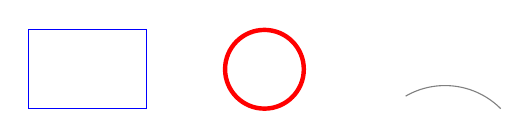
\begin{tikzpicture}
        \draw [blue] (0,0) rectangle (1.5,1);
        \draw [red, ultra thick] (3,0.5) circle [radius=0.5];;
        \draw [gray] (6,0) arc [radius=1, start angle=45, end angle= 120];
    \end{tikzpicture}

    \caption{XXX picture: Big picture}
\end{figure}

Použil jsem stochastický model postavený na individuích. Individua jsou jedinci jednoho druhu s oddělenými pohlavími a
žijí v nestrukturovaném prostředí. Fenotyp jedinců a tedy i fenotyp optimální pro dané prostředí jsou čtyřrozměrnými
vektory. Optimum prostředí $E(t)$ není stálé, ale může se měnit v čase.

Euklidovská vzdálenost fenotypu jedince od aktuálního optima prostředí určuje jeho fitness.

Optimum prostředí je po dobu 8192 kroků simulace konstantní a následně dojde k jeho skokové změně o
$\Delta{}E$. Po této změně opět zůstane optimum neměnné po dalších 8192 kroků, poté se vrátí na počáteční hodnotu.

Počáteční velikost populace je jedním z parametrů simulace. V~dalších krocích je následně velikost populace udržována
mechanismem turbidostatu.

Navíc je každý jedinec limitován maximální délkou života -- po 64 krocích umírá.
Čerstvě narození jedinci jsou sexuálně dospělí ihned v následujícím kroku simulace a věk neovliňuje jejich fenotyp.

V každém kroku jsou z populace náhodně vybrány páry opačného pohlaví.
Kolik pár vyvede potomků, je určeno průměrnou fitness páru. Způsob, jak je jsou určeny počty potomků, jejich geny a
jak následně geny určují jejich fenotyp, je popsán později.

Při každém kroku simulace také velmi malou část jedinců postihne mutace jednoho nebo více genů. Tyto mutace mají
vliv na geny, které mohou zdědit potomci jedince, jeho fenotyp však již neovlivňují a ten zůstává konstatní po celou
dobu života. Somatické mutace nejsou modelovány.

\section{Jedinec a jeho geny}

Geny každého jedince jsou uloženy v dvou homologních chromosomech. Každý z těchto chromosomů má 20 lokusů.
Na každém z lokusů je alela, která má vliv na fenotyp jedince. Alela je určena svým příspěvkem k fenotypu (čtyřrozměrný
vektor, typicky s jednou nenulovou hodnotou, tedy gen ovlivňuje jednu vlastnost jedince, dále nazýván i
\em{efekt alely}) a svým příspěvkem k fenotypu, pokud se vyskytuje na obou protilehlých lokusech
(opět čtyřrozměrný vektor, dále nazýván i \em{dominantní efekt alely}).

Na počátku simulace jsou vygenerováni náhodní jedinci. Jejich počet je parametrem simulace, zároveň je použit i jako
rovnovážná velikost populace.

Většina alel těchto jedinců má nulový příspěvek k fenotypu. Náhodně je vybráno zhruba jedno procento alel, které k
fenotypu přispívají. Jak vypadají je určeno parametry simulace - mezi nimi je, jaká je pravděpodobnost, že bude
nová alela pleiotropická a tedy ovlivňovat více složek fenotypu a jaká je pravděpodobnost,
že se u alely projeví dominance.

Pokud alela působí jen na jednu vlastnost, tak je tato vlastnost vybrána náhodně a velikost příspěvku je vybrána z
normálního rozdělení. Pokud působí na všechny složky fenotypu, tak jsou příspěvky vybrány nezávisle na sobě z normálního
rozdělení a vyděleny odmocninou z dimenze fenotypu (tedy $\sqrt{4} = 2$). Důvodem je, že bez tohoto znormování měly
pleiotropické příspěvky v průměru větší délku.

Teorie zamrzlé plasticity předpokládá podstatný význam dominantích alel, které působí v opačných směrech, pokud se
vyskytují jednou nebo dvakrát. Pravděpodobnost, že alela má takovou vlastnost je parametrem simulace.

Ostatní alely mají účinek v obou případech stejný.


Postup, jak je vygenerována každá alela v počáteční populaci tedy vypadá takto:

\begin{code}[commandchars=\\\{\}]

    pocatecni_alela() =
        \textbf{pokud} (nahodne_cislo_z_intervalu(0,1) < 0.99)
            \textbf{pak} Alela([0,0,0,0], [0,0,0,0])
            \textbf{jinak} nenulova_alela()

    nenulova_alela =
        \textbf{pokud} (nahodne_cislo_z_intervalu(0,1) < XXXX)
            \textbf{pak}
                efekt <- nahodny_jednoduchy_efekt()
                dominantni_efekt <- nahodny_dominantni_efekt(efekt)
                Alela(efekt, dominantni_efekt)
            \textbf{jinak}
                efekt <- nahodny_pleiotropicky_efekt()
                dominantni_efekt <- nahodny_dominantni_efekt(efekt)
                Alela(efekt, dominantni_efekt)

    nahodny_jednoduchy_efekt =
        zamichej([0, 0, 0, \textit{N}()])

    nahodny_jednoduchy_efekt =
        [\textit{N}() / 2, \textit{N}() / 2, \textit{N}() / 2, \textit{N}() / 2])

    nahodny_dominantni_efekt(efekt) =
        \textbf{pokud} (nahodne_cislo_z_intervalu(0,1) < jine XXXX)
            \textbf{pak} efekt
            \textbf{jinak} nahodny_opacny_efekt(efekt)

    nahodny_opacny_efekt(efekt) =
        x <- XXXX
        (-x) * efekt \textit{//násobení vektoru (záporným) skalárem}

    \textit{// {N}() značí náhodné číslo ze standardizovaného}
    \textit{//       normálního rozdělení}
    \textit{// XXXX znaci vyber z XXXX}
\end{code}

\subsection{Mutace}

Jedinou možnou mutací je bodová změna alely za jinou - nejsou tedy simulovány rozsáhlejší mutace, které mají větší vliv
na strukturu DNA.

Nad každým lokusem v obou chromosomech určeno s pravděpodobností XXX, zda u něj dojde ke změně.
V případě, že ano, tak je na lokus dána nová náhodná alela. Ta je vybírána obdobným mechanismem, jako jsou
generovny nenulové počáteční alely.

\begin{figure}
  \centering

  \begin{tikzpicture}

    \begin{scope}
      \DNASequence[Mutated]{$\blacktriangleright$/white!30,$\clubsuit$/red!30,$\#$/white!30,$\triangleleft$/white!30,$\circ$/white!30,$\flat$/white!30}
    \end{scope}

    \begin{scope}[yshift=1cm]
      \DNASequence{$\triangleright$/white!20,$\clubsuit$/white!30,$\bot$/white!20,$\triangleleft$/white!30,$\bullet$/white!30,$\sharp$/white!30}
    \end{scope}


    \begin{scope}[xshift=9cm]
      \DNASequence[Done]{$\blacktriangleright$/white!30,$\diamondsuit$/red!30,$\#$/white!30,$\triangleleft$/white!30,$\circ$/white!30,$\flat$/white!30}
    \end{scope}

    \begin{scope}[xshift=9cm,yshift=1cm]
      \DNASequence{$\triangleright$/white!20,$\clubsuit$/white!30,$\bot$/white!20,$\triangleleft$/white!30,$\bullet$/white!30,$\sharp$/white!30}
    \end{scope}

    \ConnectNodes[out=-90, in=-30]
        {Done-1.south}
        {Mutated-1.south};

  \end{tikzpicture}

  \caption{Mutace}
\end{figure}

\subsection{Křížení}

Každý jedinec má jedno ze dvou pohlaví. V každém kroku simulace jsou náhodně vytvořeny nové páry jedinců opačného
pohlaví. Jde tedy o panmiktický model populace.

Každý z potomků vzniká tak, že jsou kombinovány geny obou rodičů. Pro každý chromozom je vybrán náhodný lokus.
Lokusy před ním a on jsou naplněny alelami jednoho z rodičů, lokusy po něm alelami druhého z rodičů.

Pohlaví potomka je určeno náhodně se stejnou pravděpodobností pro obě pohlaví.

\begin{figure}
  \centering

  \begin{tikzpicture}

    \begin{scope}
      \DNASequence[Parent1a]{$\blacktriangleright$/yellow!30,$\clubsuit$/yellow!30,$\boxplus$/yellow!30,$\circ$/yellow!30,$\circledcirc$/yellow!30,$\flat$/yellow!30}
    \end{scope}

    \begin{scope}[yshift=1cm]
      \DNASequence[Parent1b]{$\triangleright$/yellow!20,$\diamondsuit$/yellow!30,$\boxdot$/yellow!20,$\bullet$/yellow!30,$\circledcirc$/yellow!30,$\flat$/yellow!30}
    \end{scope}


    \begin{scope}[yshift=3cm]
      \DNASequence[Parent2a]{$\blacktriangle$/green!30,$\clubsuit$/green!30,$\boxdot$/green!30,$\star$/green!30,$\circledcirc$/green!30,$\flat$/green!30}
    \end{scope}

    \begin{scope}[yshift=4cm]
      \DNASequence[Parent2b]{$\triangle$/green!20,$\clubsuit$/green!30,$\Box$/green!20,$\ast$/green!30,$\circledcirc$/green!30,$\sharp$/green!30}
    \end{scope}

    \begin{scope}[xshift=9cm,yshift=2cm]
      \DNASequence[Donea]{$\blacktriangle$/green!30,$\clubsuit$/green!30,$\boxplus$/yellow!30,$\circ$/yellow!30,$\circledcirc$/yellow!30,$\flat$/yellow!30}
    \end{scope}

    \begin{scope}[xshift=9cm,yshift=3cm]
      \DNASequence[Doneb]{$\triangle$/green!20,$\clubsuit$/green!30,$\Box$/green!20,$\ast$/green!30,$\circledcirc$/green!30,$\flat$/yellow!30}
    \end{scope}

    \ConnectNodes[out=-90, in=-30]
        {Donea-3.south}
        {Parent1a-3.south};

    \ConnectNodes[out=-90, in=-0]
        {Donea-0.south east}
        {Parent2a-0.south east};

    \ConnectNodes[out=90, in=40]
        {Doneb-2.north}
        {Parent2b-2.north};

    \ConnectNodes[out=90, in=40]
        {Doneb-5.north}
        {Parent1b-5.north};

  \end{tikzpicture}

  \caption{Křížení}
\end{figure}



\section{Jedinec a jeho fenotyp}

Fenotyp jedince jsou jeho čtyři kvantitativní vlastnosti dohromady reprezentované jako čtyřrozměrný vektor.

Každá alela nějak přispívá do výsledného fenotypu, tyto příspěvky se sčítají. Příspěvek alely se může lišit, pokud se
nachází ve dvou kopiích na protilehlých lokusech - v tom případě se použije její dominantní efekt.


\section{Optimum}

Pro simulovaný druh existuje optimální fenotyp, který nejlépe vyhovuje aktuálnímu stavu prostředí.
Tento optimální fenotyp se v průběhu simulace dvakrát skokově -- v jejím kroku číslo 8192 a 16384-- změní.

Počáteční optimum je nastaveno na dvanáctinásobek XXX výběru z normálního roložení nezávisle pro každou dimenzi.
První změna proběhne o dvanáctinásobek XXX  výběru z normálního rozložení nezávisle pro každou dimenzi. Druhá změna
vrátí fenotyp na půuvodní hodnotu.

XXX

\begin{equation}
E(0) =  [12{\cdot}X_1, 12{\cdot}X_2, 12{\cdot}X_3, 12{\cdot}X_4], F(X_i) \sim \phi
\end{equation}

\begin{equation}
\Delta{E} = [12{\cdot}X_1, 12{\cdot}X_2, 12{\cdot}X_3, 12{\cdot}X_4], F(X_i) \sim \phi
\end{equation}

\begin{equation}
E(t) = \left \{
     \begin{array}{l} E(0), \quad t \leq 8192 \\
                      E(0), \quad t \geq 16384 \\
                      E(0) + \Delta{E}, \quad jinak
     \end{array} \right .
\end{equation}

\subsection{Fitness}

Euklidovská vzdálenost jedince s fenotypem $X = [X_1,\dots{}X_4]$ od aktuálního optima prostředí určuje
$E = [E_1,\dots{} E_4]$ jeho aktuální fitness, tak jak bylo zavedeno ve Fisherově geometrickém modelu XXX
\footnote{Konstanta $a$ v tomto vzorci jsou čistě empiricky zvolená tak, aby, měli jedinci v simulacích
přiměřené velikosti fitness -- pokud by například místo ní byla výrazně větší konstanta, tak by pro většinu simulací
neměla většina párů potomky a druh by v nich brzy vymřel. Což je nezajímavé a neodpovídá to reálným druhům.
Dvojka v exponentu je pak ve fisherovkých modelech běžná volba[XXX].
Seznam všech konstant, jak byly voleny pro simulace, je součástí přílohy XXX.}

\begin{equation}
fitness = e^{-a |E-X|^2} = e^{-a\cdot{\sum{(E_i - X_i)^2}}}
\end{equation}

Počet potomků páru je aritmetický průměr fitness jeho členů zaokrouhlený dolů.


\section{Řízení velikosti populace}

Počáteční velikost populace je jedním z parametrů simulace.
\footnote{Seznam všech parametrů simulace je součástí přílohy XXX}
Následně je velikost populace řízena turbidostatickou
zpětnou vazbou[XXX]. V každém kroku má v populaci s $n$ jedinci každý jedinec pravděpodobnost
$p = min(0.9, k_4 n^2 + k5)$, že zahyne. Člen $k_4 n^2$ závisí na čtverci velikosti populace, a tedy její hustotě.
V přírodě mu odpovídá například regulace parazitem, kterému se lépe daří, pokud se jedinci častěji setkávají.
Člen $k5$ je pravděpodobnost náhodného úmrtí nezávislého na velikosti populace. Pravděpodobnost je z praktických důvodů
zastropována hodnotou 0.9 -- bez tohoto omezení by mohla s $n$ růst nade všechny meze a tedy i nad $1.0$, kde se ztrácí
možnost (nejen biologické) interpretace.
\footnote{Vzorec pro turbidostatickou regulaci očividně odpovídá realitě jenom pro aktuální velikosti populace,
které řádově nepřekračují rovnovážnou velikost populace. Omezení pravděpodobnosti pod $0.9$ v představovaných
simulacích postačuje pro postupný pokles k očekávané velikosti populace, protože počet potomků je omezený a
menší než deset na pár.}

Konstanta $k4$ v předchozím vzorci je vypočítána následově:

\begin{equation}
k_4 = \frac{4 - 12\cdot{}{k_5} - \frac{12}{a_{max}}}
           {27\cdot{}n^2}
\end{equation}


kde $n_0$ je rovnovážná velikost populace a $a_{max}$ je maximální věk jedince.
Pro simulace byla zvolena nulová pravděpodobnost náhodného úmrtí $k5$ a řízení velikosti populace tedy záviselo jen na
její hustotě a na deterministické smrti stářím po $a_{max}$ generacích.

Vzorec pro velikost $k_4$ je poněkud neintuitivní, ale dá se odvodit z požadavku, aby velikost populace zůstala
konstantní za předpokladu konstantní průměrné fitness:

\begin{equation}
(k_4\cdot{m^2} + {k_5} + \frac{1}{a_{max}})\cdot{m} = m - n
\end{equation}

kde $m$ je aktualní velikost populace po množení, $a_{max}$ je věk, ve kterém umírají organismy stářím a $n$ je rovnovážná
velikost populace. Vzorec říká, že pro rovnovážnou velikost by měl být počet úmrtí (což je počet úmrtí daný
turbidostatem plus počet úmrtí stářím) stejný jako počet čerstv narozených jedinců.

\begin{equation}
m = n + \frac{n\cdot{}p}{2}
\end{equation}

kde $p$ je průměrná pravděpodobnost, že pár vyvede v daném kole mládě. (Párů je v populaci zhruba $\frac{n}{2}$, protože
obě pohlaví jsou zhruba stejně zastoupena).


Odtud:

\begin{equation}
(k_4\cdot{(n + \frac{n\cdot{}p}{2})^2} + {k_5} + \frac{1}{a_{max}})\cdot{(n + \frac{n\cdot{}p}{2})}
        = n + \frac{n\cdot{}p}{2}  - n
\end{equation}

\begin{equation}
(k_4\cdot{(n + \frac{n\cdot{}p}{2})^2} + {k_5} + \frac{1}{a_{max}})\cdot{(n + \frac{n\cdot{}p}{2})} = \frac{n\cdot{}p}{2}
\end{equation}

\begin{equation}
(k_4\cdot{(n + \frac{n\cdot{}p}{2})^2} + {k_5} + \frac{1}{a_{max}})\cdot{(2 + p)} = p
\end{equation}


\begin{equation}
(k_4\cdot{(n + \frac{n\cdot{}p}{2})^2} + {k_5} + \frac{1}{a_{max}}) - \frac{p}{(2 + p)}
\end{equation}

\begin{equation}
k_4\cdot{(n + \frac{n\cdot{}p}{2})^2} = \frac{p}{2 + p} -  {k_5} - \frac{1}{a_{max}}
\end{equation}

\begin{equation}
k_4  = \frac{\frac{p}{2 + p} -  {k_5} - \frac{1}{a_{max}}}{(n + \frac{n\cdot{}p}{2})^2}
\end{equation}


Vzorec můžeme chápat jako funkci proměnné $p$ (průměrné pravděpodobnosti rozmnožení páru), což nelze použít  pro
počáteční inicializaci simulace, kdy $p$ není známa. Budeme tedy uvažovat rovnováhu populace v jednom konkrétním
případě - pokud je optimálně přizpůsobena prostředí a pak je $p = 1.0$. Pokud nebude populace dokonale přizpůsobena
prostředí, bude ji turbidostat udržovat méně početnou.

Dosazením a úpravou lze získat:



\begin{equation}
k_4  = \frac{\frac{1}{2 + 1} -  {k_5} - \frac{1}{a_{max}}}{(n + \frac{n\cdot{}1}{2})^2}
     = \frac{\frac{1}{3} -  {k_5} - \frac{1}{a_{max}}}{(n + \frac{n}{2})^2}
     = \frac{\frac{1}{3} -  {k_5} - \frac{1}{a_{max}}}{(\frac{3\cdot{}n}{2})^2}
\end{equation}

\begin{equation}
k_4  = \frac{\frac{1}{3} -  {k_5} - \frac{1}{a_{max}}}{\frac{9\cdot{}n^2}{4}}
     = \frac{\frac{4}{3} - 4\cdot{}{k_5} - \frac{4}{a_{max}}}{9\cdot{}n^2}
\end{equation}

\begin{equation}
k_4  = \frac{4 - 12\cdot{}{k_5} - \frac{12}{a_{max}}}{27\cdot{}n^2}
\end{equation}

\section{Frozen Beagle}

Popsaná simulace byla implementována v silně staticky typovaném čistě funkcionálním jazyce Haskell \citep{Haskell}.

Samotná simulace je zapouzdřena do knihovny, která je užívána dvěma programy -- grafickým
\textit{FrozenBeagleSimulation} a \textit{fbeagle}, který je spouštěn z příkazové řádky.

Grafický \textit{FrozenBeagleSimulation}, zobrazený na XXX,
umožňuje pohodlně nastavit parametry simulace a jednu spustit.



%\begin{figure}
%\centering
%\includegraphics[totalheight=8cm]{img/ukazka-obr01.pdf}
%    \caption{FrozenBeagleSimulation screenshot}
%\end{figure}


\textit{fbeagle} je vhodný pro dávkové zpracování, které spouští mnoho simulací se stejnými parametry, které se liší
počátečním \textit{seedem} generátoru pseudonáhodných čísel. Jeho výstupem je sada statistik pro jednotlivé simulace,
které je moźné dále analyzovat a zpracovávat.

Na adrese \url {https://github.com/satai/FrozenBeagle} jsou volně k dispozici zdrojové texty včetně jednotkových testů
a kompletní historie ve VCS git. Jsou poskytnuty pod trojsložkovou BSD licencí.

\section{Statistická analýza}

\section{Reprodukovatelnost}

Bla, bla.

K sazbě byl použit systém \TeX se sadou maker \LaTeX a za použití fontů Latin Modern.
